\msusection{Panels Menu}\label{sec:panels}
Three additional panels for manipulating data within YCweather are available: Thermocouple Plotter, Add Logs and Images, and Search.  These features are available via the Panels menu on the Program Control window.  These panels may be triggered automatically when YCweather opens via the program Preferences (Section \ref{sec:pref}).  Figure \ref{fig:panels} shows the Program Control window with all the panels.  Each of these panels servers a specific function, as defined below, that a typical user will likely not require.

\begin{figure}[h]\centering
	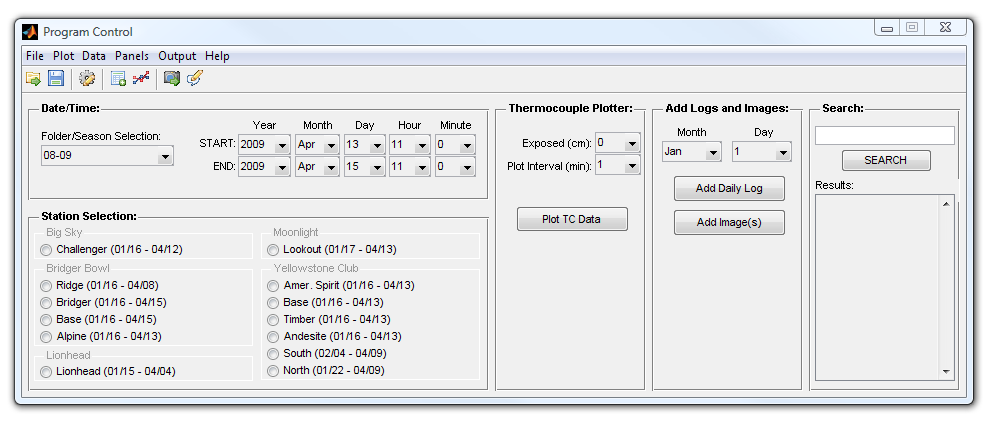
\includegraphics[width=\linewidth]{\YCfiles figures/panels.png}
	\caption{Program Control with all side panels showing.}
	\label{fig:panels}
\end{figure}

\msusubsection{Thermocouple Plotter}
A weather station may contain thermocouple data that extends into the snowpack, such as the North and South stations at the Yellowstone Club.  In this case it is desirable to graph temperature profiles of the snow pack at various intervals; the Thermocouple Plotter panel serves this purpose.  To understand this feature consider the following tutorial, referring to Figure \ref{fig:TCexample}.

\begin{enumerate}
	\item Open the Yellowstone Club South weather station Data List, as in Figure \ref{fig:TCexample}.  In the Data List window a list of thermocouple will be present in the Temperature panel, this indicates that this station has thermocouple data.
	\item Open the Thermocouple Plotter panel using the Panels menu on the Program Control window.
	\item Select a start and end time on the Program Control for just a few hours as in Figure \ref{fig:TCexample}.
	\item Change the Plot Interval pop-up menu to 30 minutes on the Thermocouple Plotter panel.
	\item Change the Exposed pop-up menu to a value of four.
	\item Press the Plot TC Data button.
\end{enumerate}

\begin{figure}[ht!]\centering
	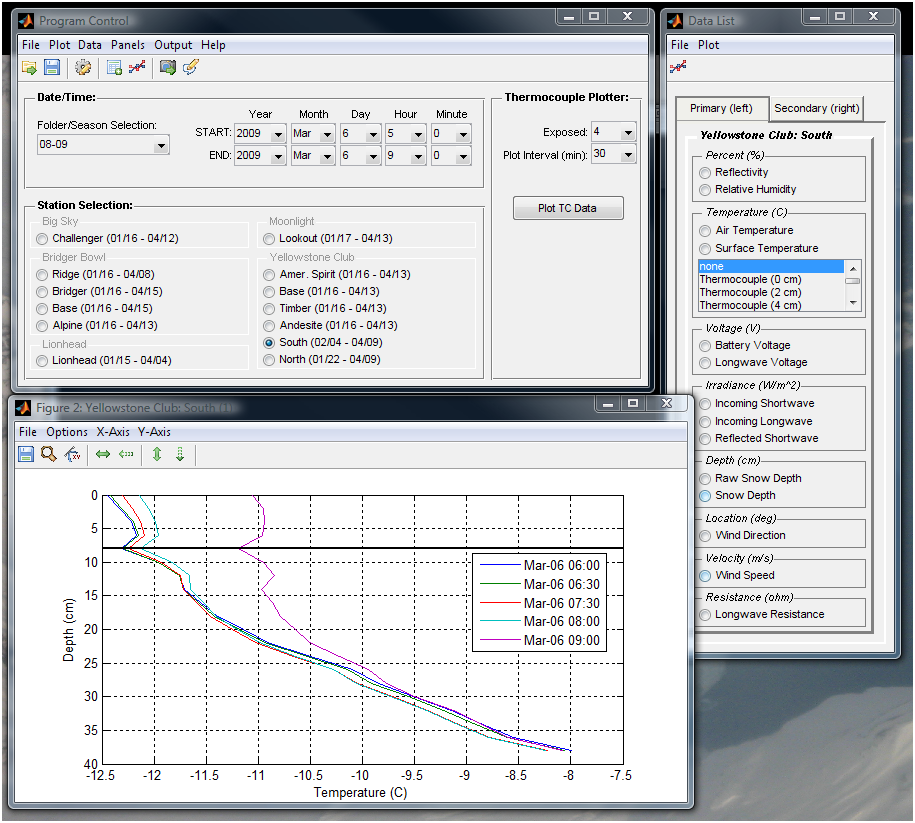
\includegraphics[width=\linewidth]{\YCfiles figures/TCexample.png}
	\caption{Example workspace showing a graph of thermocouple data.}
	\label{fig:TCexample}
\end{figure}

Following the above steps should produce a graph similar to that displayed in Figure \ref{fig:TCexample}.  This graph displays the theromocouple profiles at 30 minute intervals over the specified time.  The horizontal black line is meant to represent the snow surface.  For the North and South Yellowstone Club weather stations the number of thermocouples exposed is recorded in the daily logs.

\msusubsection{Add Logs and Images}\label{sec:add}
This panel allows the user to add image files and daily logs to a specific station for a specific date.  Each weather station (e.g. South at the Yellowstone Club or Ridge at Bridger Bowl) may have images and a daily log associated with the station for each day.  The Add Logs and Images panel allows this data to be assigned.  For example, to add a daily log for February 13 at the South Yellowstone Club station:
\begin{enumerate}
	\item select the South station from the Yellowstone Club panel in the Program Control window,
	\item select the appropriate day from the Add Logs and Images panel, and
	\item press the \q{Add Daily Log} button.
\end{enumerate}

Performing these steps opens a window for adding and editing the daily log.  Enter the desired information and then select the Save daily log option from the File menu.  If a log already exists for the selected station and date, a warning will appear.  If it is desired to overwrite the log then continue, otherwise the log should be edited.  Editing daily logs is discussed in \ref{sec:dailylogs}.

Similarly, images can be added to the YCweather database.  In this case the program will prompt the user to select the desired images to include, these images will be added to the database and accessible via the image viewer.  No changes to the images occur, YCweather simply builds a reference to the image file(s).  For specifics on the YCweather file organization within the database see Section \ref{sec:advanced}.

\msusubsection{Search}
The Search panel provides the user a tool for searching all the daily log (Section \ref{sec:dailylogs}) files for a specific folder/season.  Type the desired keyword(s) in the window with multiple words separated by a comma.  If any matches for any of the keywords exist the station and date will appear in the Results list.  Selecting the desired result opens the associated daily log.
